\section{Theory}

The method of this study is being made possible from the theory described in this section. This section will cover all theory surrounding the building and testing the prototype built in this thesis. These theories are: 
\begin{itemize}
  \item Design
  \item Design software
  \item Web development
  \item Programming languages
  \item Distributing software
  \item Testing methodologies. 
\end{itemize}



% \textit{Don't know were to put this}
% \subsection{Relationship Between Designer and Developer}%
% \label{sub:Relationship Between Designer and Developer}
% To create a great product the collaboration between designers and developers is essential.

% \textit{"Without the proper alignment and synergy of skillsets, the user experience you provide your users will lack efficiency, engagement, and value."} - Khamdamova, \cite{RelationshipDesignersDevelopers} 

\subsection{Design}%
\label{sub:Design}
The design work is primarily done at the start of the project. After that, the project team contacts the customer and hash out what functionality and appearance the application will have. However, it is often problematic for customers to know what they want and what is possible with software. Therefore this design segment is often done in iterations. 

A fairly common way of designing a website is to first create prototypes with low fidelity. Then add more details to the prototype through iterations until the design is of high fidelity and could be mistaken for an actual website. 

The medium with which these prototypes are created varies, but a \acrfull{ui} design application is often used to make the final high fidelity prototype. This high-fidelity prototype is accurate with the final product meaning that all colors, typographies, and layout are complete. The developer then translates the design prototype into a functional website.

\subsubsection{UI Design Applications}%
\label{ssub:Apps}
\acrshort{ui} design is often the first step in building an application. By designing the \acrshort{ui} first, the designer can collaborate with the customer iteratively until they have a design agreed upon to move forward to development.

Sketch\cite{sketchDigitalDesignToolkit} was released in 2010 and was one of the first applications that mainly focused on \acrshort{ui} design. In later years applications such as Figma\cite{figmaFigmaCollaborativeInterface}  (released 2016) and Adobe XD\cite{adobeAdobeXDFast} (released 2015) have come to overtake Sketch's dominance\cite{SketchVsFigma0200}. 

In this thesis, Figma is the \acrshort{ui} design application that is used because Knowit is already using this tool. Figma is also one of few design applications with an open \acrshort{rest}-\acrshort{api} that gives access to all prototype elements. This makes the project possible because all design data is accessible for a third-party tool that can create functional web components.  

 
% Since the early 10's the UI design applications have been around to make this easier.


% Assesemnt of Figma vs Sketch \cite{SketchVsFigma0200} 




\subsubsection{Figma}%
\label{sub:Figma}
Figma is a vector-based \acrshort{ui} Design application that is web-based, which means that the whole software is run over a network\cite{FigmaCollaborativeInterface} . 

Figma has an open \acrshort{rest}-\acrshort{api} (Representational State Transfer) that supplies the information of the Figma document to servers over the Internet\cite{figmaFigma, RepresentationalStateTransfer2021}. Figma was chosen as the \acrshort{api} design application since it is web-based and Knowit uses it today. The \acrshort{api} is then updated after each design change, which is great for collaboration and keeping the \acrshort{rest}-\acrshort{api} updated.

\paragraph{Figma Components}%
\label{ssub:Figma Components}
Figma allows its users to create \glspl{component}. A \gls{component} is, as explained earlier, a set of fundamental elements that are combined. Figures \ref{fig:images/cardComp} and \ref{fig:images/cardCompElements} show an example of a card\cite{babichSimpleDesignTips2020} \gls{component} in Figma. The card \gls{component} consists of four elements, two text elements, and two frame elements. 

\begin{figure}[H]
  \centering
  \begin{minipage}[b]{0.48\textwidth}
    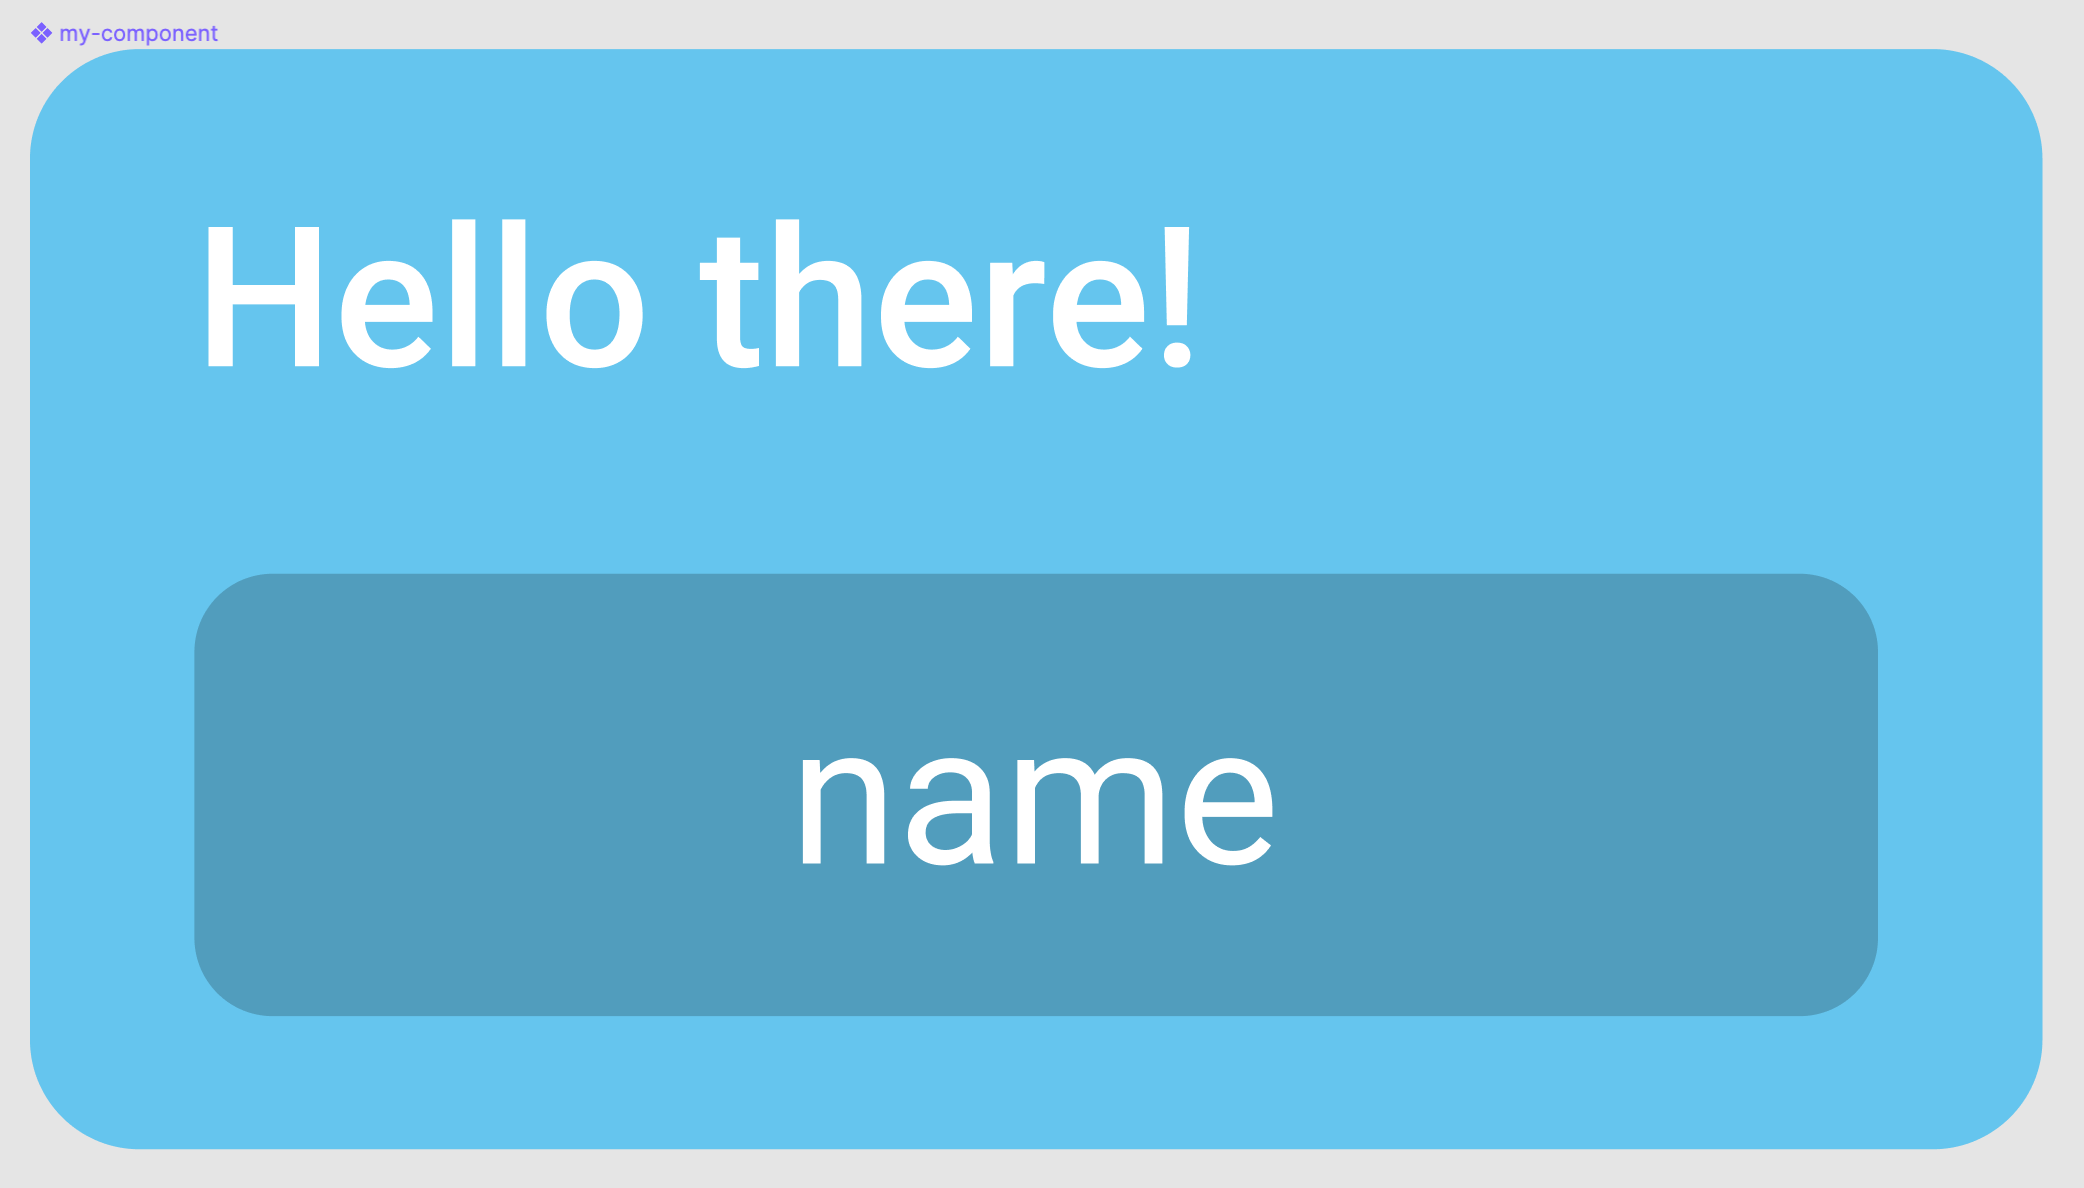
\includegraphics[width=\linewidth]{images/cardComp.png}
    \caption{Figma component}
    \label{fig:images/cardComp}
  \end{minipage}
  \hfill
  \begin{minipage}[b]{0.48\textwidth}
    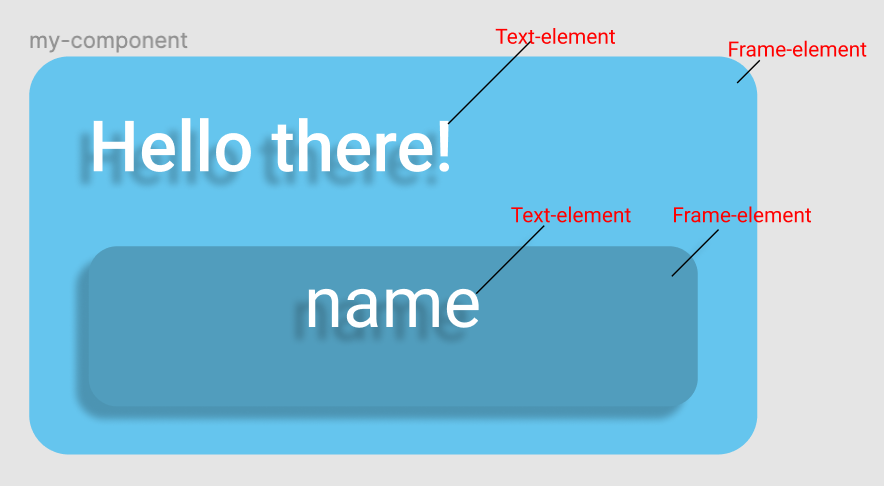
\includegraphics[width=\linewidth]{images/cardCompElements.png}
    \caption{Elements of a component}
    \label{fig:images/cardCompElements}
  \end{minipage}
\end{figure}


When copying a \gls{component}, the copied \gls{component} is \textit{attached} to the original \gls{component}. When making changes to the original \gls{component}, all \textit{attached} \glspl{component} will get the updates. The attached \glspl{component} can be changed without affecting the original \gls{component}. 

\paragraph{Figma Styles}%
\label{ssub:Styles}

Figma has a feature that lets the user store colors, texts, and effects as \textit{styles}. This is a way for the user to store default styles for their design.  For example, if the default color for a design is green, the user can store this green color as a color style. The user can use the color style throughout their \acrfull{ui}. If they later want to change the default color for the \acrshort{ui}, they only need to change the color of the color \textit{style}, not all colored elements individually. The changes between Figures \ref{fig:images/layoutBlue} and \ref{fig:images/layoutGreen} are from changing the color style. The same principle extends to typographies and effects such as shadows and blurs. 

\begin{figure}[H]
  \centering
  \begin{minipage}[b]{0.48\textwidth}
    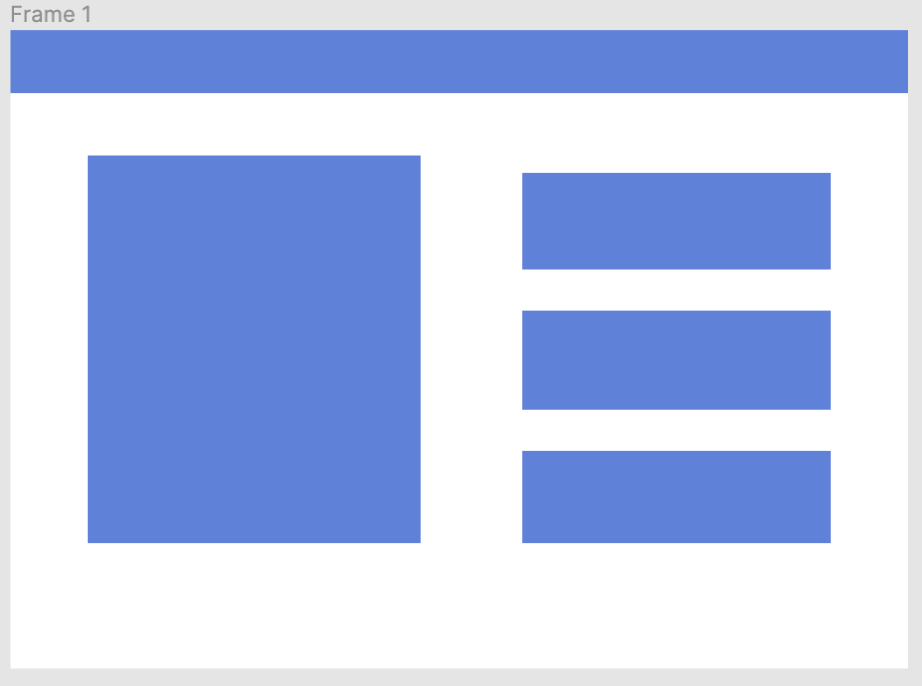
\includegraphics[width=\linewidth]{images/layoutBlue.png}
    \caption{UI with blue color style}
    \label{fig:images/layoutBlue}
  \end{minipage}
  \hfill
  \begin{minipage}[b]{0.48\textwidth}
    
\includegraphics[width=\linewidth]{images/layoutGreen.png}
    \caption{UI with green color style}
    \label{fig:images/layoutGreen}
  \end{minipage}
\end{figure}



% \subsection{Competitors}%
% \label{sub:Competitors}
% The idea of making a design program generate functional code is not new. In this section some of the competitors of this genre of programs will be brought up and compared.

% \subsubsection{Webflow}
% Webflow was founded in 2013 and is a product from the famous program Y Combinator. Webflow allows the user to design, create and publish a website all from their program. Webflow is, as Figma, a network based application that works form a web browser. 



% Webflows website: \cite{ResponsiveWebDesign} 

% \subsubsection{Visly}%
% \label{ssub:Visly}
% Visly website: \cite{vislyVisly} 
% Visly is was founded in 2018 and is very similar to Figma in how the user designs the product. Visly uses the design to create React components \cite{facebookincReactJavaScriptLibrary}. React is a component based JavaScript framework made by Facebook. Visly essentially makes it possible to create these components visually.

% \subsubsection{Bravo}%
% \label{ssub:Bravo}

% Build Native IOS och Android apps with Figma. Think this can be the closest to the what I'm trying to do. 

% \subsubsection{Comparison}%
% \label{ssub:Comparison}



% \subsubsection{Components}%
% \label{sub:Components}



\subsection{Develop}%
\label{sub:Develop}

A website is usually built using the three main languages of the web: \acrfull{html}, CSS, and JavaScript. \acrshort{html} is a \textit{''tagging''} language meaning all code is written with tags. All information is written between or in opening and closing tags. An opening tag signifies a tag with  <\textit{nameOfTag}> and a closing tag </\textit{nameOfTag}>. Attributes can be assigned within the opening tag, such as a class or an id.  
\acrshort{html} is often referred to as the body of a website. This is where the majority of the information on the web pages is stored. \acrshort{css} is the clothes to the body. \acrshort{css} is what defines the style for the website, such as sizes, paddings, and colors.\\
\textit{"\acrshort{css} describes how \acrshort{html} elements are to be displayed on screen, paper, or in other media"} - W3school.com\cite{CSSIntroduction}.\\
JavaScript is a scripting language that enables the developer to create complex features on web pages. JavaScript enables us to update the content of the website dynamically. 

In modern web design, many different frameworks, libraries, and, languages make it easier for developers to create products.  All these tools have one thing in common. They all convert their design to the three standard browser languages, \acrshort{html}, \acrshort{css}, and JavaScript. 

One of the thesis objectives is to create a tool that could be used in as many projects as possible.  


\subsubsection{REST API}%
\label{sub:REST API}
\gls{rest} stands for \textbf{Re}presentational \textbf{S}tate \textbf{T}ransfer and is an architectural style of distributed hypermedia systems. Roy Fielding created this in 2000 with the release of his dissertation\cite{fieldingFieldingDissertationCHAPTER}. An \acrshort{api} to be called RESTful needs to fill the following six requirements\cite{fieldingFieldingDissertationCHAPTER,restfulapi.netWhatREST}. 

\begin{enumerate}
  \item Client-server - the UI and data storage are separated. 
  \item Stateless - The server does not store any information about the client. The client must provide all information for every request. 
  \item Cacheable - A response can be explicitly or implicitly labeled as cacheable or non-cacheable. If the response is cacheable, the client has the right to store and reuse the response data for later. 
  \item Uniform interface - Simplifies and decouples the architecture between clients and servers, which enables each part to evolve independently.  
  \item Layered system - This architecture consists of hierarchical layers that constrain what each component can do, such as; a component can only interact with the layer it is on. 
  \item Code on demand (optional) - This allows the client to download and execute applets or scripts and therefore extending client functionality 
\end{enumerate}

These requirements make the \acrshort{api} lightweight and easy to understand and introduce fewer problems into the system. 


\subsubsection{JavaScript and TypeScript}%
\label{ssub:JavaScript and TypeScript}
JavaScript is a programming language that reports its error much later than many other languages. This is because variables can take any shape in JavaScript. That is, for instance, a number or a string. This can at first seem promising, that the language is highly dynamic and flexible. However, this flexibility is also very error-prone, where most of the errors are discovered after the code is run. Because of this, the developer is obliged to test running the code after every change\cite{taivalsaari2008web}. TypeScript was created to fix the error-prone nature of JavaScript. TypeScript is an open-source superset of JavaScript. TypeScript allows for the creation of types for variables, functions, etc., and thereby helps to find more errors before runtime\cite{WhyYouShould}. TypeScript then complies back to JavaScript before it is run and can thereby run everywhere JavaScript is run\cite{WhyYouShould}. 


% \textit{Incremental testing is required. Due to its highly permissive, error-tolerant nature, JavaScript programming requires an incremental, evolutionary approach to testing as well. Since errors are reported much later than usual, by the time an error is reported it is often surprisingly difficult to pinpoint the original location of the error. Error detection is made harder by the dynamic nature of JavaScript, for instance, by the option to change some of the system features on the fly. Furthermore, in the absence of strong, static typing, it is possible to execute a program and only at runtime realize that some parts of the program are missing. For all these reasons, the best way to write JavaScript programs is to proceed step by step, by writing (and immediately testing) each new piece of code. If such an incremental, evolutionary approach is not used, debugging and testing can become quite tedious even for relatively small JavaScript applications.} 



\subsubsection{Node.js}%
\label{ssub:Node}
Node.js is an open-source project that lets its users run code on the server asynchronously\cite{node.js}. JavaScript is a single-threaded language, meaning that the compiler runs the program from top to bottom. If a function is dependent on another function, the latter function needs to wait for the first function to finish. This is called blocking and can become frustrating for the user\cite{GeneralAsynchronousProgramming}. For example, an application has a flow of scrollable pictures and a button for saving a picture on the cloud. If this is implemented incorrectly and blocking occurs, the user will not be able to scroll through new pictures until the application has completed the process of saving the image. Using asynchronous programming blocking can be avoided by running the different functions on different threads, which is what node.js does. This allows for a more efficient way of running JavaScript code without a browser. Node.js is designed to handle HTTP effectively. Streaming and low latency have therefore been a high priority. 


\subsubsection{Syntactically Awesome Style Sheets (SASS)}%
\label{sub:sass}
\acrfull{sass} is an extension language to \acrshort{css} that adds more functionality to regular \acrshort{css}. With \acrshort{sass}, it is possible to have a stylesheet split up into multiple files, create functions, etc. \acrshort{sass} is then compiled to regular \acrshort{css} so the browser can understand it. \acrshort{sass} is also called a preprocessor for \acrshort{css} because of this. \acrshort{sass} has two different syntaxes; the indented syntax, commonly referred to as \acrshort{sass}, and sassy \acrshort{css}, referred to as \acrshort{scss}. The indented syntax was the original syntax for \acrshort{sass} and is only dependent on indentation. \acrshort{scss} syntax is very similar to regular \acrshort{css} but with the qualities of \acrshort{sass}. Because of the resemblance of standard \acrshort{css}, \acrshort{scss} is the more popular of the two syntaxes. For these reasons \acrshort{scss} will be used in this project.


\paragraph{Variables}
Variables in a stylesheet are helpful, especially when dealing with colors. Often websites have color schemes from their design. By assigning each color to a variable, only one row of code needs to be changed if the color scheme is updated. Regular \acrshort{css} does support variables, but they can be cumbersome to use, especially if the variables will be used globally in the stylesheet.

To style an element in \acrshort{css}, we must first target the element with a \acrshort{css} selector. A selector could be an HTML element such as a div or a heading. \acrshort{css} also has additional selectors called \glspl{pseudo}. \Glspl{pseudo} are defined by a colon before their name, such as :after, :before, and :root. These elements do not add additional data to the website but help the developer to style it. 

A variable in \acrshort{css} is defined by adding two dashes before the variable name.  The variable must also be defined within a selector and thereby only operate within that selector. The :root \gls{pseudo} can be used to define variables globally within the stylesheet. When using the variables, they must be put inside the var()-function to work.
Below an example of defining and using a variable can be seen. 

\begin{lstlisting}[style=htmlcssjs]

:root{
  --myColorVariable: #ff9a67; 
}

div{
  background-color: var(--myColorVariable);
}
\end{lstlisting}


\acrshort{scss} variables are not required to be defined within a selector, making them globally reachable within the stylesheet by default. The dollar-sign (''\$'') is used to define an \acrshort{scss} variable. We can use an \acrshort{scss} variable by simply adding the variable where we want to use it. The example below is achieving the same result as the previous example.


\begin{lstlisting}[style=htmlcssjs]
\$myColorVariable: #ff9a67; 

div{
  background-color: \$myColorVariable;
}
\end{lstlisting}


\paragraph{Mixin and Include}
\acrshort{css} is notoriously known for having numerous code duplications. These duplications occur when different elements need the same subset of \acrshort{css} rules. \acrshort{scss} has a solution to this, called \glspl{mixin}. A \gls{mixin} is a function that stores multiple \acrshort{css} rules defined with @mixin before the function name and used with @include. Below is an example of centering all children in an element with a \gls{mixin}. 

\begin{lstlisting}[style=htmlcssjs]
@mixin centered {
  display: grid;
  place-items: center;
}; 

div{
  @include centered; 
}
\end{lstlisting}

% \subsubsection{CSS Methodologies}%
% \label{ssub:methodologies}

% Explanation for BEM\cite{contributorsBEMBlockElement} 

% \subsubsection{SCSS}%
% \label{ssub:SCSS}
% \cite{\acrshort{sass}SyntacticallyAwesome} 

% \subsubsection{Webpack}%
% \label{sub:Webpack}





\subsubsection{Web Components}%
\label{sub:Web Components}
Web Components are a set of different JavaScript \acrshortpl{api} and \acrshort{html} features that make it possible to create reusable custom elements\cite{WebComponentsMDN}. These elements are encapsulated away from the rest of the code. All major browsers support these web components. Because web components are run natively on \acrshort{html}, \acrshort{css}, and JavaScript, they are compatible with all JavaScript frameworks, such as React, Vue, and Angular. Web components are built with three technologies: Custom elements, shadow DOM, and \acrshort{html} Templates. 

\paragraph{Custom Elements}
With the help of a set of JavaScript \acrshortpl{api}, we can define custom elements and their behavior. By creating custom elements, we can encapsulate \acrshort{html} functionality outside of the main page itself. By doing this, the \acrshort{html} code becomes much more readable. 

\paragraph{Shadow DOM}%
\label{ssub:Shadow DOM}
When the browser reads in an \acrshort{html} page, a document object model tree (\acrshort{dom} tree) is created.  In figure \ref{fig:shadow}, we can see this tree. Shadow \acrshort{dom} is a set of JavaScript \acrshortpl{api} that lets us attach an encapsulated ''shadow'' \acrshort{dom} tree to an existing node in the \acrshort{dom} tree. This ''shadow'' \acrshort{dom} extends the main document \acrshort{dom} like a branch. The difference from a regular branch is that the main \acrshort{dom} is not aware of the ''shadow'' \acrshort{dom}s data or functionality and vice versa. The ''shadow'' \acrshort{dom} is then essentially its own tree with its own stylesheet that cannot be modified or overwritten from the main \acrshort{dom}.\\
\begin{figure}[H]
  \centering
  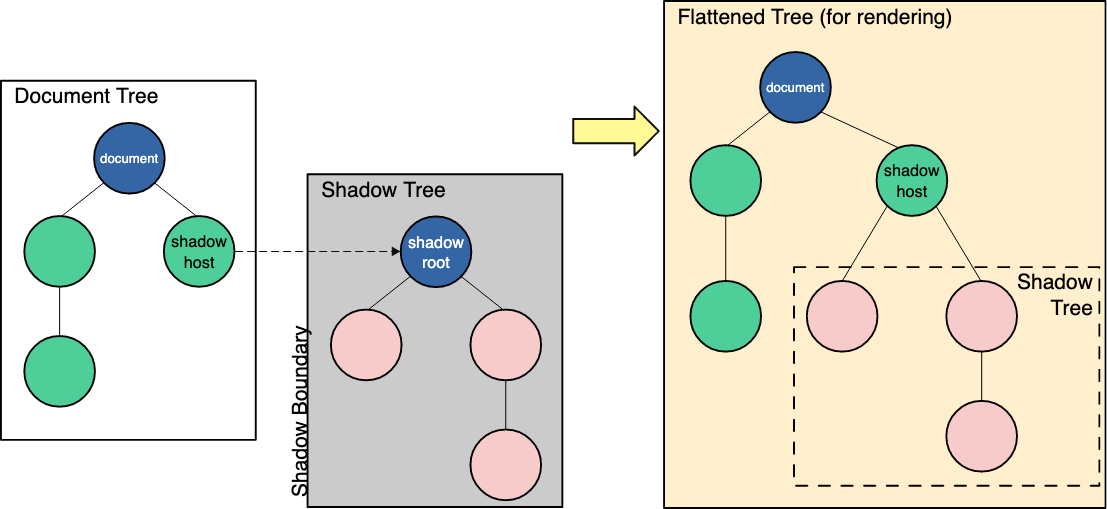
\includegraphics[width=0.8\linewidth]{images/shadow.png}
  \caption{Depiction of a shadow DOM attached to the main DOM}%
  \label{fig:shadow}
\end{figure}




\paragraph{HTML Templates}%
\label{ssub:HMTL Templates}
The \acrshort{html} \textit{template}-tag and \textit{slot}-tag enable the developer to write markup templates that are not displayed on the rendered \acrshort{html} page. These templates can then be reused throughout the \acrshort{html} page. \acrshort{html} templates enable web components to be reused multiple times, with different instances, in the \acrshort{dom} tree


\subsubsection{LitElement}%
\label{ssub:LitElement}
Web components can be manually built using custom elements, shadow \acrshort{dom}, and \acrshort{html} templates mentioned above. A group of engineers from the Google Chrome team in the Polymer Project \cite{polymerPolymerProject} created a lightweight JavaScript class called LitElement. LitElement combines functionality from the web components technologies to a class that makes it easy to create web components with concise and malleable code.


% \subsubsection{Recursive functions}%
% \label{ssub:Recursive functions}
% A small but very powerful caviat of programming is recursive fucntions. This is when a funcions calls itself inside said function.






\subsection{Distribute}%
\label{sub:Distribute}
After a \gls{component} has been designed and developed, the \glspl{component} can now be used in a project. Often the created \gls{component} is used by more than one part, and therefore it should be distributed seamlessly. There are many ways to distribute a \gls{component}, but the most widely used way is to use a package manager.


% To be able to use the components created from the designer the developers need to be able to get a hold of them. A lot of reusable code that is crated for the web can be accessed from the internet with the help of package managers.
\subsubsection{Package Manager}%
\label{sub:Package Manager}
% \cite{PackageManager2020} 

The most traditional way of installing and updating software is by downloading an installer. The installer will then install the software to the system. Then, if an update is needed, the software can notify the user to update or update itself in the background. 

A package manager can install and update software with ease compared to a more traditional installer. A package manager bundles up the source code into a package. This package can then be distributed over the Internet and installed and updated without an internal installer. 

The package manager that this project will use is \acrfull{npm}, which is the world's largest software registry\cite{NpmNpmDocs}.
\acrshort{npm} has a straightforward interface, whereas if something needs to be installed, the following can be typed in the terminal: 

\begin{lstlisting}[style=htmlcssjs]
\$npm install PACKAGE-NAME
\end{lstlisting}

\subsubsection{Open Source}%
\label{ssub:Open Source}

\textit{"The term open source refers to something people can modify and share because its design is publicly accessible."} - Opensource.com\cite{WhatOpenSource}

Open source originated from developers creating software that was designed to be open and modified by anyone. In an open-source project, the source code for the software must be available for others to use. To signify that the project is open-source, an open-source license is added to the source code. These licenses affect how the user can use, study, distribute, and modify the software's source code. The most used licenses state that the user can do anything they wish with the software. Some licenses state that if alterations are done on the software, the altered version must also be open-source. 

% \subsection{Semi-Structured Interviews}%
% \label{sub:inteviews}
% This tool is involved with people in many different areas of expertise, form designers to front-end developers to back-end developers. To get a clear view of of how these people work to create the best tool for them the semi-structured interview was used. 

% For collecting data from the employees of Knowit semi-structured interviews were used \cite{galletta2013mastering}. 





\subsection{Testing}%
\label{sub:Testing}
When a product has been created, tests can be run on the product. The test's main objective is to find contingent bugs in the software and flaws with the UI. Further, the testing is done to ensure that assumptions taken when creating the product are verified or debunked.

\subsubsection{Usability testing}%
\label{ssub:User testing}
Usability testing or "user research" is a broad term. As Lewis\cite{lewis2006usability} described it: "Usability testing, in general, involves representative users attempting representative tasks in representative environments, on early prototypes or working versions of computer interfaces." 

Usability testing is essentially performed to find flaws in an interface by putting the user in the environment of using the interface. Usability testing is done in all stages of development, from paper prototypes to high-fidelity screen mock-ups to the finished product. 

Lazar et al.\cite[Chapter~10]{lazar2017research}  consider usability testing a cousin to traditional research methods, where traditional research refers to methods such as experimental design\cite[Chapter~3]{lazar2017research}  and ethnography\cite[Chapter~9]{lazar2017research}.
Similarities can be found in experimental design with measurement of task performance and time performance, surveys, and observation techniques from ethnography. The participants in usability testing, as in traditional research, must remain anonymous, be informed of their rights, and can leave the research at any time. What separates usability testing from traditional research is often the end goals. For usability testing, the end goals are to create the best product possible, with the time and resources at hand, while the traditional research methods want to find answers to questions that are universal for the field researched. 
	
Wixson proclaims in his study that usability testing is closer to engineering than traditional research \cite{wixon2003evaluating}. Usability testing, as engineering, is focused on creating a successful product with limited time and resources. Tests are done in iterations where the prototype will be changed between each test to fix the flaws found during the test. The next iteration of tests will then be used to verify the fixed flaws simultaneously as it searches for other flaws. This is, in most if not all traditional research, considered unacceptable. This because there is no way of knowing or statistically verifying the results from the first tests. 

To get more credible data out of a test and not just for improving the product, the test environment should be kept as similar as possible for each user. By doing this, the data can be statistically analyzed, making it easier to make more accurate decisions of what to do next.

Usability testing can collect quantitative data such as time- and task performance. However, the majority of data that is collected is qualitative. As mentioned before, the most significant end goal for a usability test is to uncover flaws in the user interface, which is often subjective for the user. 

\textit{"Often in industry, schedule and resource issues, rather than theoretical discussions of methodology, drive the development process \cite{wixon2003evaluating}."}

\paragraph{Sufficient Amount of Test Users}
\label{ssub:Sufficient Amount of Test Users}

In usability testing, it has become widely accepted that five users are the most efficient number of participants for usability testing.  Nielsen and Landauer suggest the number five out of a cost ratio to numbers of tests\cite{nielsen1993mathematical}. Nielsen started the \textit{''discount usability movement''} in 1989 with his presentation of the paper: "Usability Engineering at a Discount"\cite{experienceDiscountUsability20}. This \textit{movement} tries to find cost-effective methods for usability testing. 
From Nielsen and Landauer's study, they found that the number of usability problems found in a usability test with n users is:
\[ N (1-(1- L ) n ) \]

Where \textit{N} is the total number of usability problems and  \textit{L} is the proportion of problems found by one test user. With this, they determined that when using five users, 80\% of usability problems are found.

Lazar, et al. explains that many researchers disagree with the assertion of five test users for successful usability testing because of Nielsen and Landauer approximation of the total number of usability problems\cite[Chapter~10.5.3]{lazar2017research}. This number \textit{N} is probably unknown, and therefore the number of test users \textit{n} cannot be found.

The topic of what number of test users are sufficient for usability testing has been discussed for over 30 years. What is important to point out is that performing usability testing is more valuable to do than not to do. 


\textit{
So instead of saying, “how many users must you have?,” maybe the correct question is “how many users can we afford?,” “how many users can we get?” or “how many users do we have time for?”
} \cite{lazar2017research} 



% \cite{nielsen1994estimating} 

% \cite{nielsen1994heuristic} 




\subsubsection{A/B Testing}%
\label{sub:A/B Testing}
% A/B testing, or bucket testing, is a user experience (UX) research method where two variants of a program/interface are tested. These two variants are referred to as A and B, hence the name A/B testing. The A and the B variant are tested on the user and then their responses are compared and evaluated. Often just a small change is made in a UI and evaluated on a lot of people 
 
% A/B testing is verified using two-sample hypothesis testing from the field of statistics. This means that decisions be made completely based on data. Then there is no guessing on where to go next.

A/B testing, or bucket testing, is a statistical method often used in \acrfull{ux} research where two variants of a program/interface are tested. These two variants are referred to as A and B, hence the name A/B testing. The A and the B variant are tested on the user, and then their responses are compared and evaluated. Often just a small change is made in a \acrshort{ui} and evaluated on many users. 

A/B testing is verified using two-sample hypothesis testing from the field of statistics. This means that decisions that will be made are entirely based on data. Then there is no guessing on where to go next.

To explain this further, we will use an example.
This example will follow five steps: 
\begin{enumerate}
  \item Identifying the goal of the test. 
  \item What will be tested? 
 \item Create a ''control'' and ''challenger''. 
 \item Split users into equally large sample groups.
 \item Decide how significant the result of the test needs to be.
\end{enumerate}
 
In this example, we will use an user interface of a data management application, see figure \ref{fig:images/A}. 

\begin{figure}[H]
  \centering
  \begin{minipage}[b]{0.45\textwidth}
    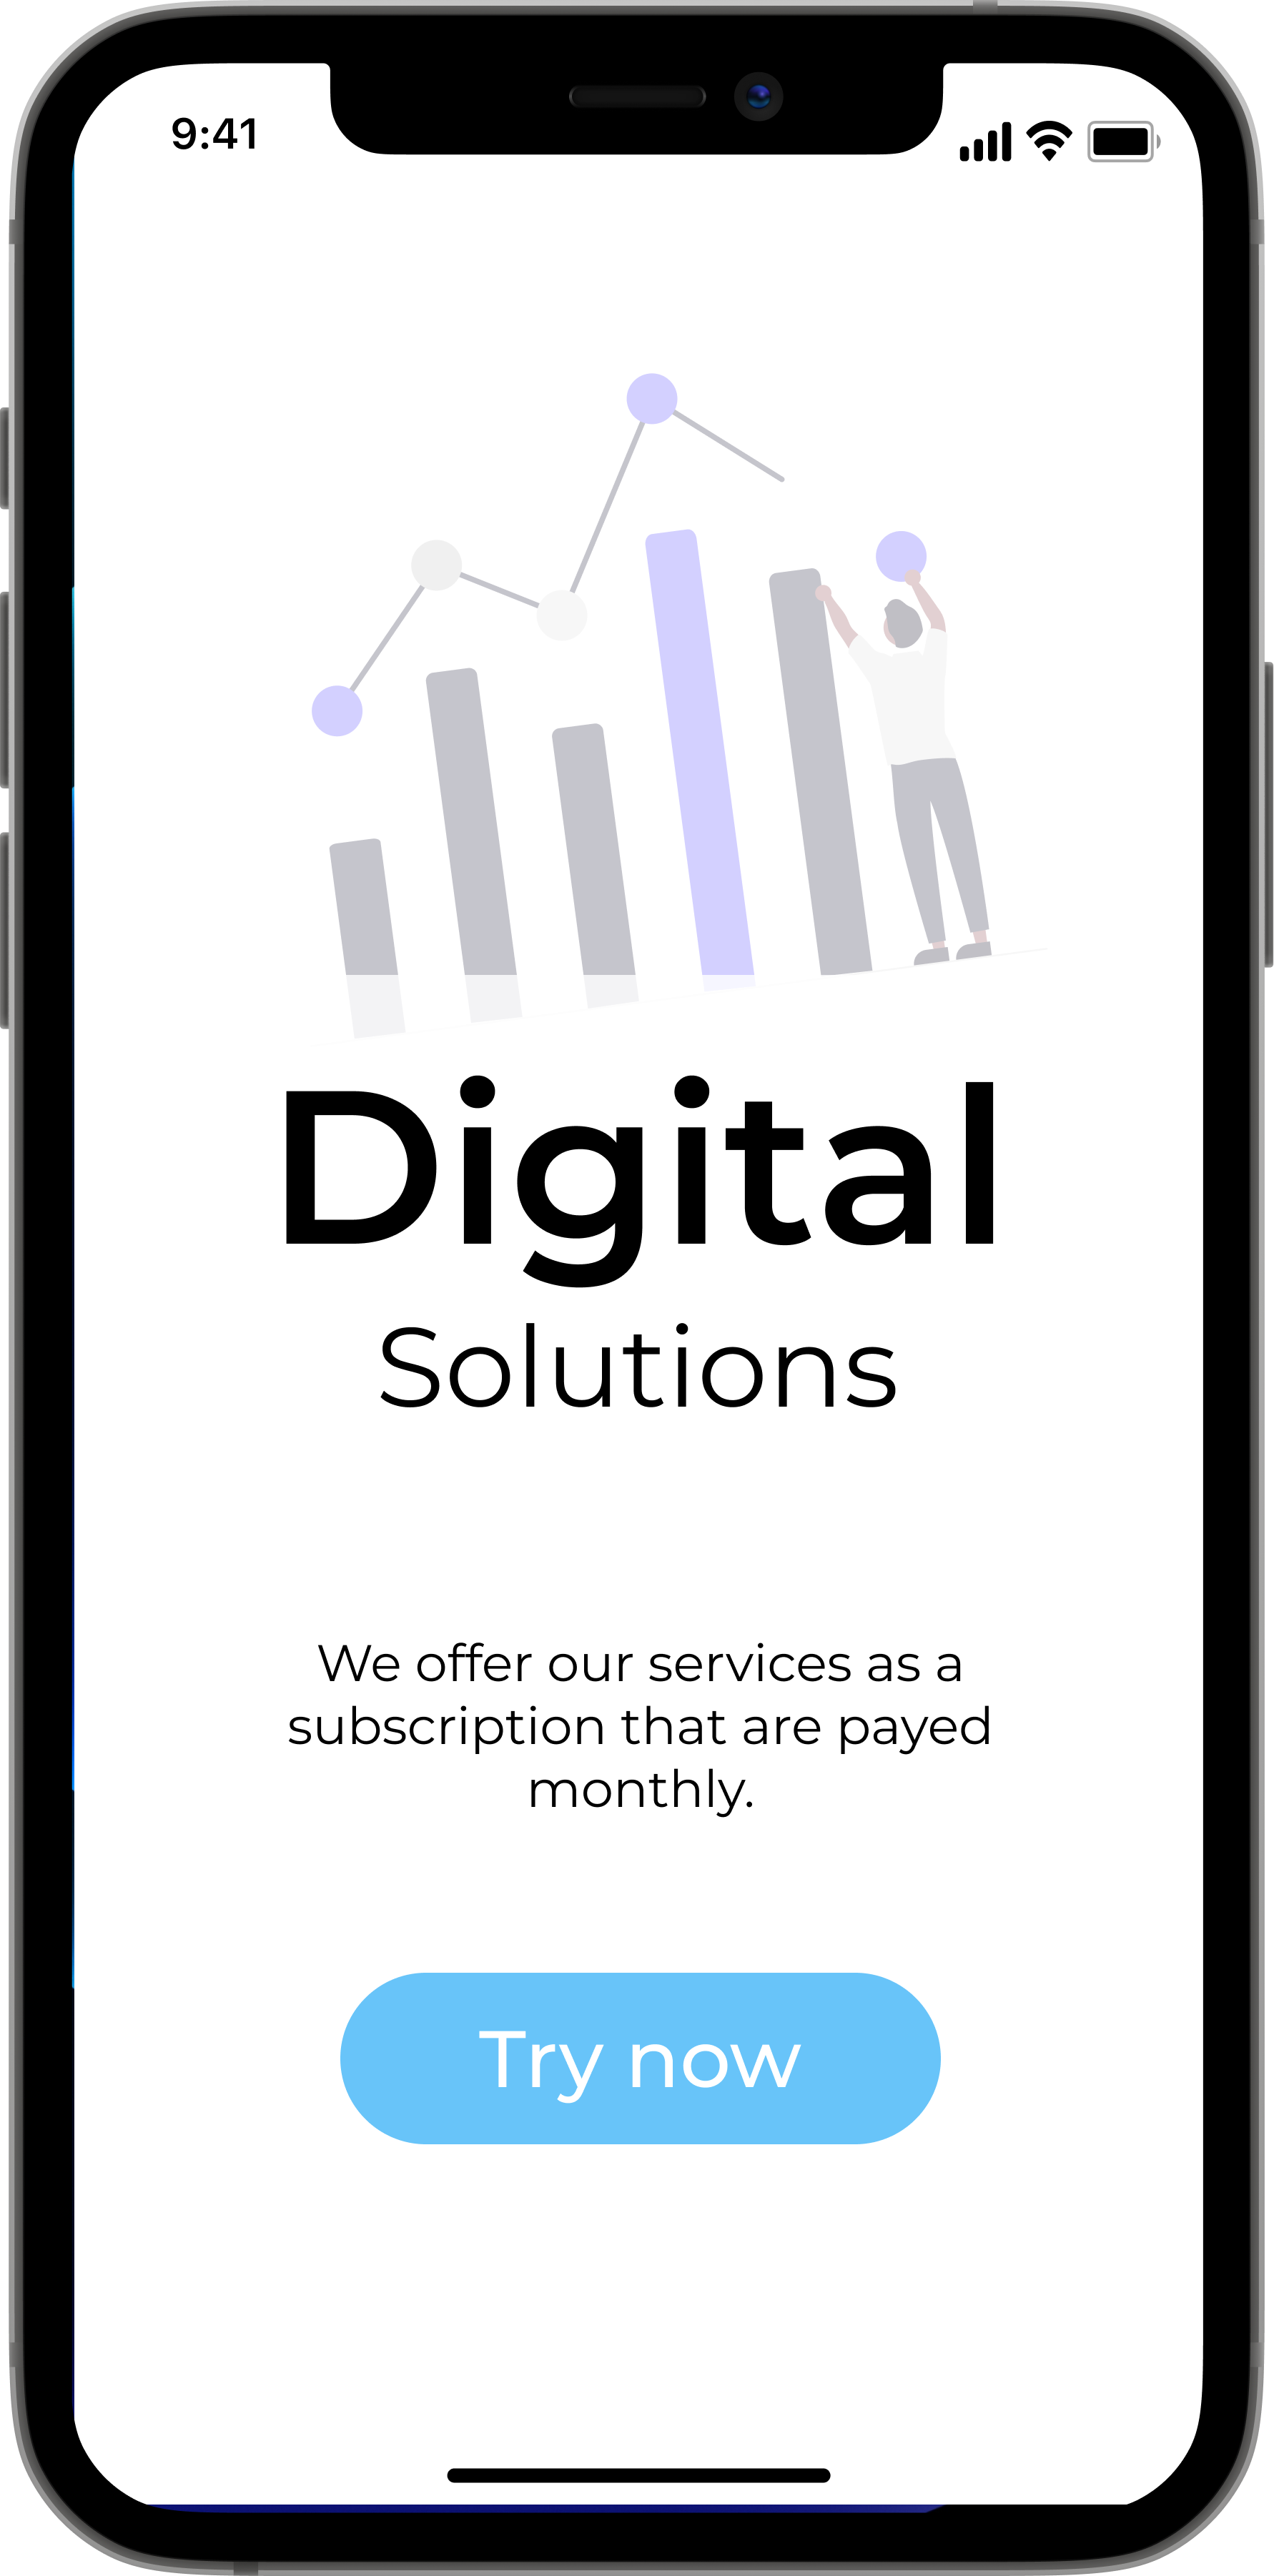
\includegraphics[width=\linewidth]{images/A.png}
    \caption{Variant A for the A/B-test}
    \label{fig:images/A}
  \end{minipage}
  \hfill
  \begin{minipage}[b]{0.45\textwidth}
    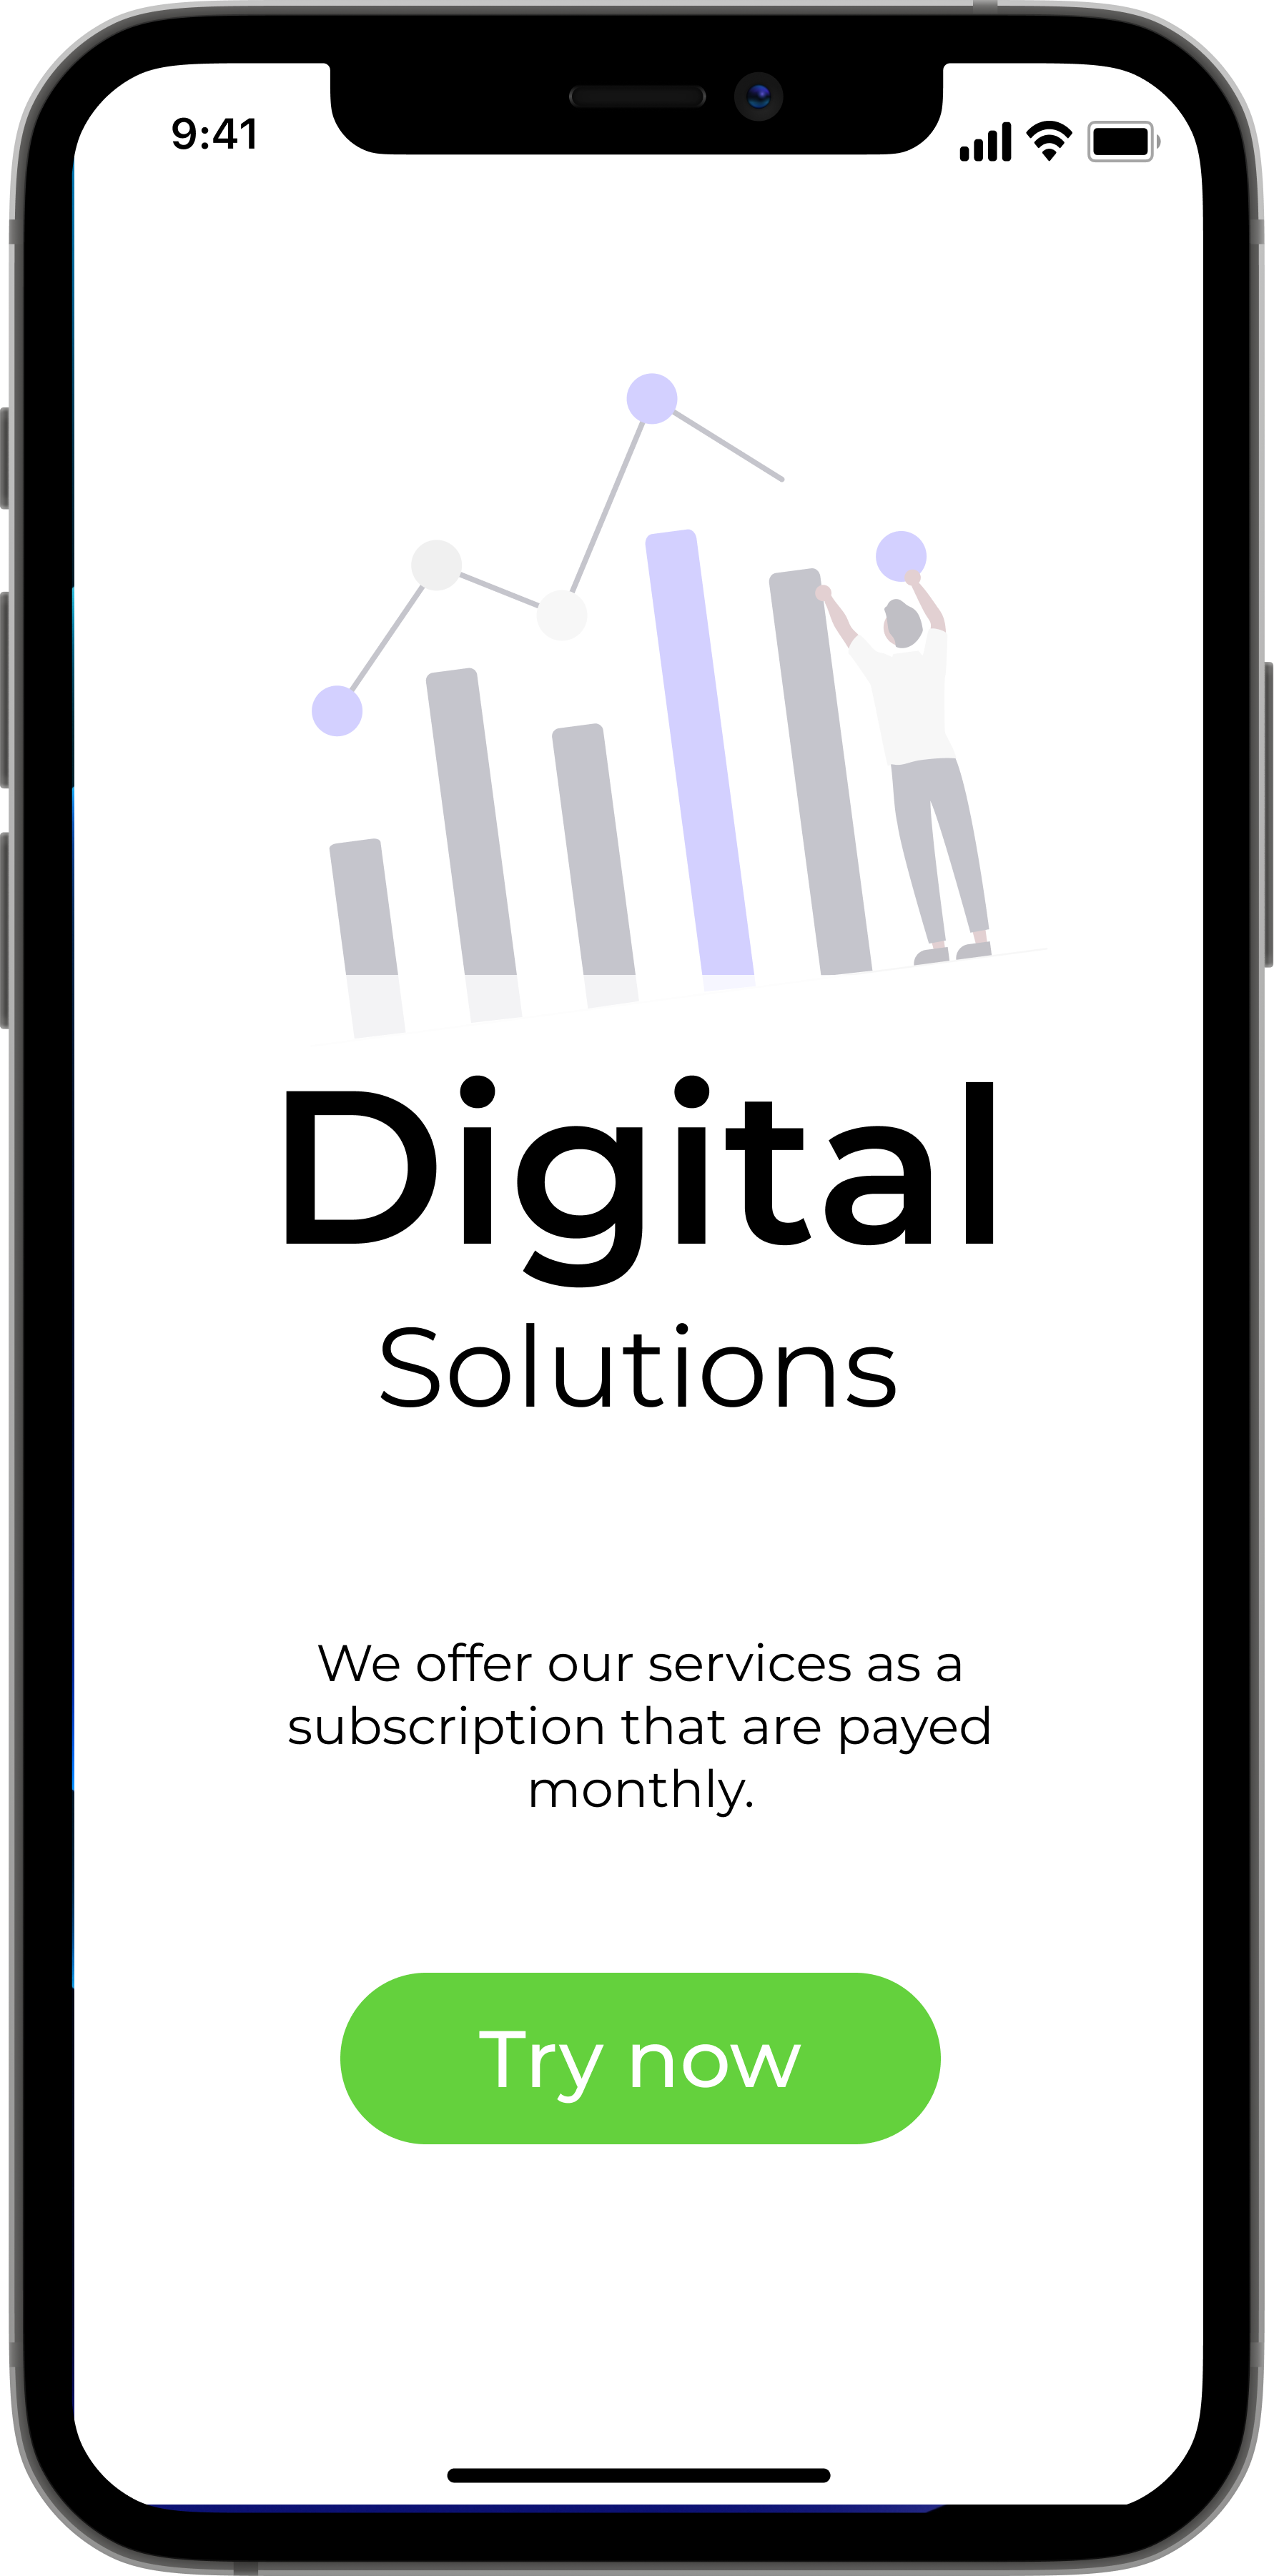
\includegraphics[width=\linewidth]{images/B.png}
    \caption{Variant B for the A/B-test}
    \label{fig:images/B}
  \end{minipage}
\end{figure}

\textbf{Identifying goal} \\
We want more users to try the digital solutions in the application. Therefore the goal for the test will be to optimize the click rate on the ''Try now'' button.

\textbf{What will be tested?}\\
We will only focus on the color of the ''Try now'' button. This is the only change that will be done. Because of this, we can be sure what effect the color of the button has on click rate. 

\textbf{Create a ''control'' and ''challenger''. }\\
The two variants tested are often called the ''control'' and the ''challenger''. In our example, the ''control'', which has not changed, is variant A and the ''challenger'' is variant B, which has a green button instead of blue. These variants can be seen in figures \ref{fig:images/A} and \ref{fig:images/B}.

\textbf{Split users into sample groups.}\\
The users are split into equally large sample groups where they either are shown variant A or variant B. 

\textbf{Decide how significant the result of the test needs to be.}\\
Before the test begins, a statistical significance must be established. Usually, this number is set to 95\%-99\%, meaning a 5\%-1\% chance that the test is showing a false positive. A false positive is a test result that wrongly indicates that a particular condition or attribute is present. For example, if a person tests positive for Covid-19 without actually having the disease.



Our hypothesis for the test is that variant B will get a higher click rate than variant A. We run the test on 20000 users, where 10000 gets variant A, and 10000 gets variant B. We record every time a user presses the button.In table \ref{tab:ab}, we can see a small portion of these recordings.

\begin{table}[H]
  \centering
\begin{tabular}{|l|l|l|}
\cline{1-3} 
        & Group & Pressed \\\cline{1-3} 
user 1  & A     & yes     \\\cline{1-3} 
user 2  & A     &         \\\cline{1-3} 
user 3  & B     & yes     \\\cline{1-3} 
user 4  & A     &         \\\cline{1-3} 
user 5  & B     &         \\\cline{1-3} 
user 6  & B     & yes     \\\cline{1-3} 
user 7  & A     &         \\\cline{1-3} 
user 8  & B     & yes     \\\cline{1-3} 
user 9  & A     & yes     \\\cline{1-3} 
user 10 & B     & yes     \\\cline{1-3}  
\end{tabular}
\caption{Table of a sample of users.}
\label{tab:ab}
\end{table}

To establish the significance value for the test, we remove all values in the \textit{group} column. Then we can simulate the group for each user, e.g., randomly apply a group to each user. 

% \begin{table}[H]
% \begin{tabular}{|l|l|l|l|l|l|l|l|l|l|l|}
% \cline{1-3} \cline{5-7} \cline{9-11}
%         & Group & Pressed &                  &         & Group & Pressed &                  &         & Group & Pressed \\ \cline{1-3} \cline{5-7} \cline{9-11} 
% user 1  & A     & yes     &                  & user 1  &       & yes     &                  & user 1  & A     & yes     \\ \cline{1-3} \cline{5-7} \cline{9-11} 
% user 2  & A     &         &                  & user 2  &       &         &                  & user 2  & A     &         \\ \cline{1-3} \cline{5-7} \cline{9-11} 
% user 3  & B     & yes     &                  & user 3  &       & yes     &                  & user 3  & A     & yes     \\ \cline{1-3} \cline{5-7} \cline{9-11} 
% user 4  & A     &         &                  & user 4  &       &         &                  & user 4  & B     &         \\ \cline{1-3} \cline{5-7} \cline{9-11} 
% user 5  & B     &         & --\textgreater{} & user 5  &       &         & --\textgreater{} & user 5  & A     &         \\ \cline{1-3} \cline{5-7} \cline{9-11} 
% user 6  & B     & yes     &                  & user 6  &       & yes     &                  & user 6  & B     & yes     \\ \cline{1-3} \cline{5-7} \cline{9-11} 
% user 7  & A     &         &                  & user 7  &       &         &                  & user 7  & A     &         \\ \cline{1-3} \cline{5-7} \cline{9-11} 
% user 8  & B     & yes     &                  & user 8  &       & yes     &                  & user 8  & B     & yes     \\ \cline{1-3} \cline{5-7} \cline{9-11} 
% user 9  & A     & yes     &                  & user 9  &       & yes     &                  & user 9  & B     & yes     \\ \cline{1-3} \cline{5-7} \cline{9-11} 
% user 10 & B     & yes     &                  & user 10 &       & yes     &                  & user 10 & B     & yes     \\ \cline{1-3} \cline{5-7} \cline{9-11} 
% \end{tabular}
% \caption{Table over the test and removed AB}
% \label{tab:abProg}
% \end{table}


By doing this simulation, a distribution of the combination of A and B can be observed. When the distribution is known, we can estimate the probability of all A and B combinations. In our example, we saw that in the empirical test, two users in group A pressed the button, and four users in group B pressed the button.  We then look at our simulated distribution of what probability there is that the empirical test results or more extreme occurred.  


\subsubsection{Statistical Analysis}%
\label{sub:Statistical analysis}
When data has been collected a statistical analysis needs to be done to be able to make any ''hard'' conclusions. A lot of decisions need to be made when analyzing the collected data. What statistical method to be used, the confidence threshold, and how the interpretation and significance of the test results should be. If the wrong method is used or if the interpretation of the results is inappropriate the conclusions drawn from the study can be erroneous \cite{lazar2017research}. 


\textbf{Preparing Data:} before we can do anything with the data often the data must be cleaned and organized.\\
\textbf{Descriptive statistic:} when the data has been cleaned and organized it can be a good idea to run some tests to understand the nature of the data. This can unfold what patterns or tendencies lays in the data. This makes it easier to choose the correct statistical method for the collected data at hand.\\
% Skillnad mellan analys och resultat: Analys = laga mat, Resultat = servera mat.
\textbf{Analyze:} when we understand the nature of the data we can analyze the data with the help of a statistical analysis method. This method could be a T- or F-tests, chi-squared test, etc. depending on the data collected.\\ 
\textbf{Results:} when the analysis is done the results must be interpreted according to the methods used.\\


% \paragraph{Preparing Data}%
% \label{ssub:Preparing Data}
% \textbf{Cleaning data}
% \textbf{Organizing}

% \paragraph{What does the data look like?}%
% \label{ssub:data look like}
% \textbf{Tendency's}
% \textbf{Patterns}
% \textbf{What statistical method should be used?}

% \paragraph{Analyze and compare}%
% \label{ssub:Analyze and compare}

% \paragraph{Summary and results}%
% \label{ssub:Summary and results}

% \begin{itemize}
%   \item Preparing data
%     \begin{itemize}
%       \item Cleaning data
%       \item Organizing 
%     \end{itemize}
%   \item What does the data look like?
%     \begin{itemize}
%       \item Tendency's
%       \item Patterns
%       \item What methods should be used?
%     \end{itemize}
%   \item Analyze and compare
%   \item Summary and results
% \end{itemize}


